
\noindent\begin{minipage}{\textwidth}
    \begin{table}[H]
        \centering
        \caption{Hiperparâmetros e Resultados do Melhor Modelo - swin\_v1\_AB\_opt}
        \vspace{0.2cm}
        \resizebox{\textwidth}{!}{%
            \begin{tabular}{ll | lrrr}
                \hline
                \multicolumn{2}{c|}{\textbf{Hiperparâmetros}} & \multicolumn{4}{c}{\textbf{Métricas por Classe}} \\ \hline
                \textbf{Parâmetro} & \textbf{Valor} & \textbf{Classe} & \textbf{Precisão} & \textbf{Recall} & \textbf{F1-Score} \\ \hline
    Agendador (Patience) & 6 & 31.2 & 0,4539 & 0,2832 & 0,3488 \\ 
Agendador de LR & ReduceLROnPlateau & 31.3 & 0,0000 & 0,0000 & 0,0000 \\ 
Architecture & swin\_s & 31.4 & 0,1768 & 0,1381 & 0,1551 \\ 
Batch Size & 32 & 32.3 & 0,2264 & 0,0612 & 0,0964 \\ 
Decaimento de Peso (WD) & 0,0348 & 32.4 & 0,0000 & 0,0000 & 0,0000 \\ 
Dropout & 0,0992 & 33.3 & 0,2042 & 0,2021 & 0,2031 \\ 
Função de Perda & CrossEntropyLoss & 41.4 & 0,0591 & 0,3182 & 0,0996 \\ 
Hidden Units & 512 & 41.5 & 0,1608 & 0,5897 & 0,2527 \\ 
Label Smoothing & 0,0931 & 42.4 & 0,0994 & 0,2353 & 0,1397 \\ 
Otimizador & AdamW & 44.4 & 0,0898 & 0,5172 & 0,1531 \\ 
\cline{3-6} 
Taxa de Aprendizado (LR) & 1,18e-04 & \textbf{Média (Macro)} & 0,2158 & 0,2090 & 0,1542 \\ 
Unfreeze Layers & 3 & \textbf{MCC} & \multicolumn{3}{c}{0,1443} \\ 
            \hline
            \end{tabular}%
        }
    \end{table}

    \begin{figure}[H]
        \centering
        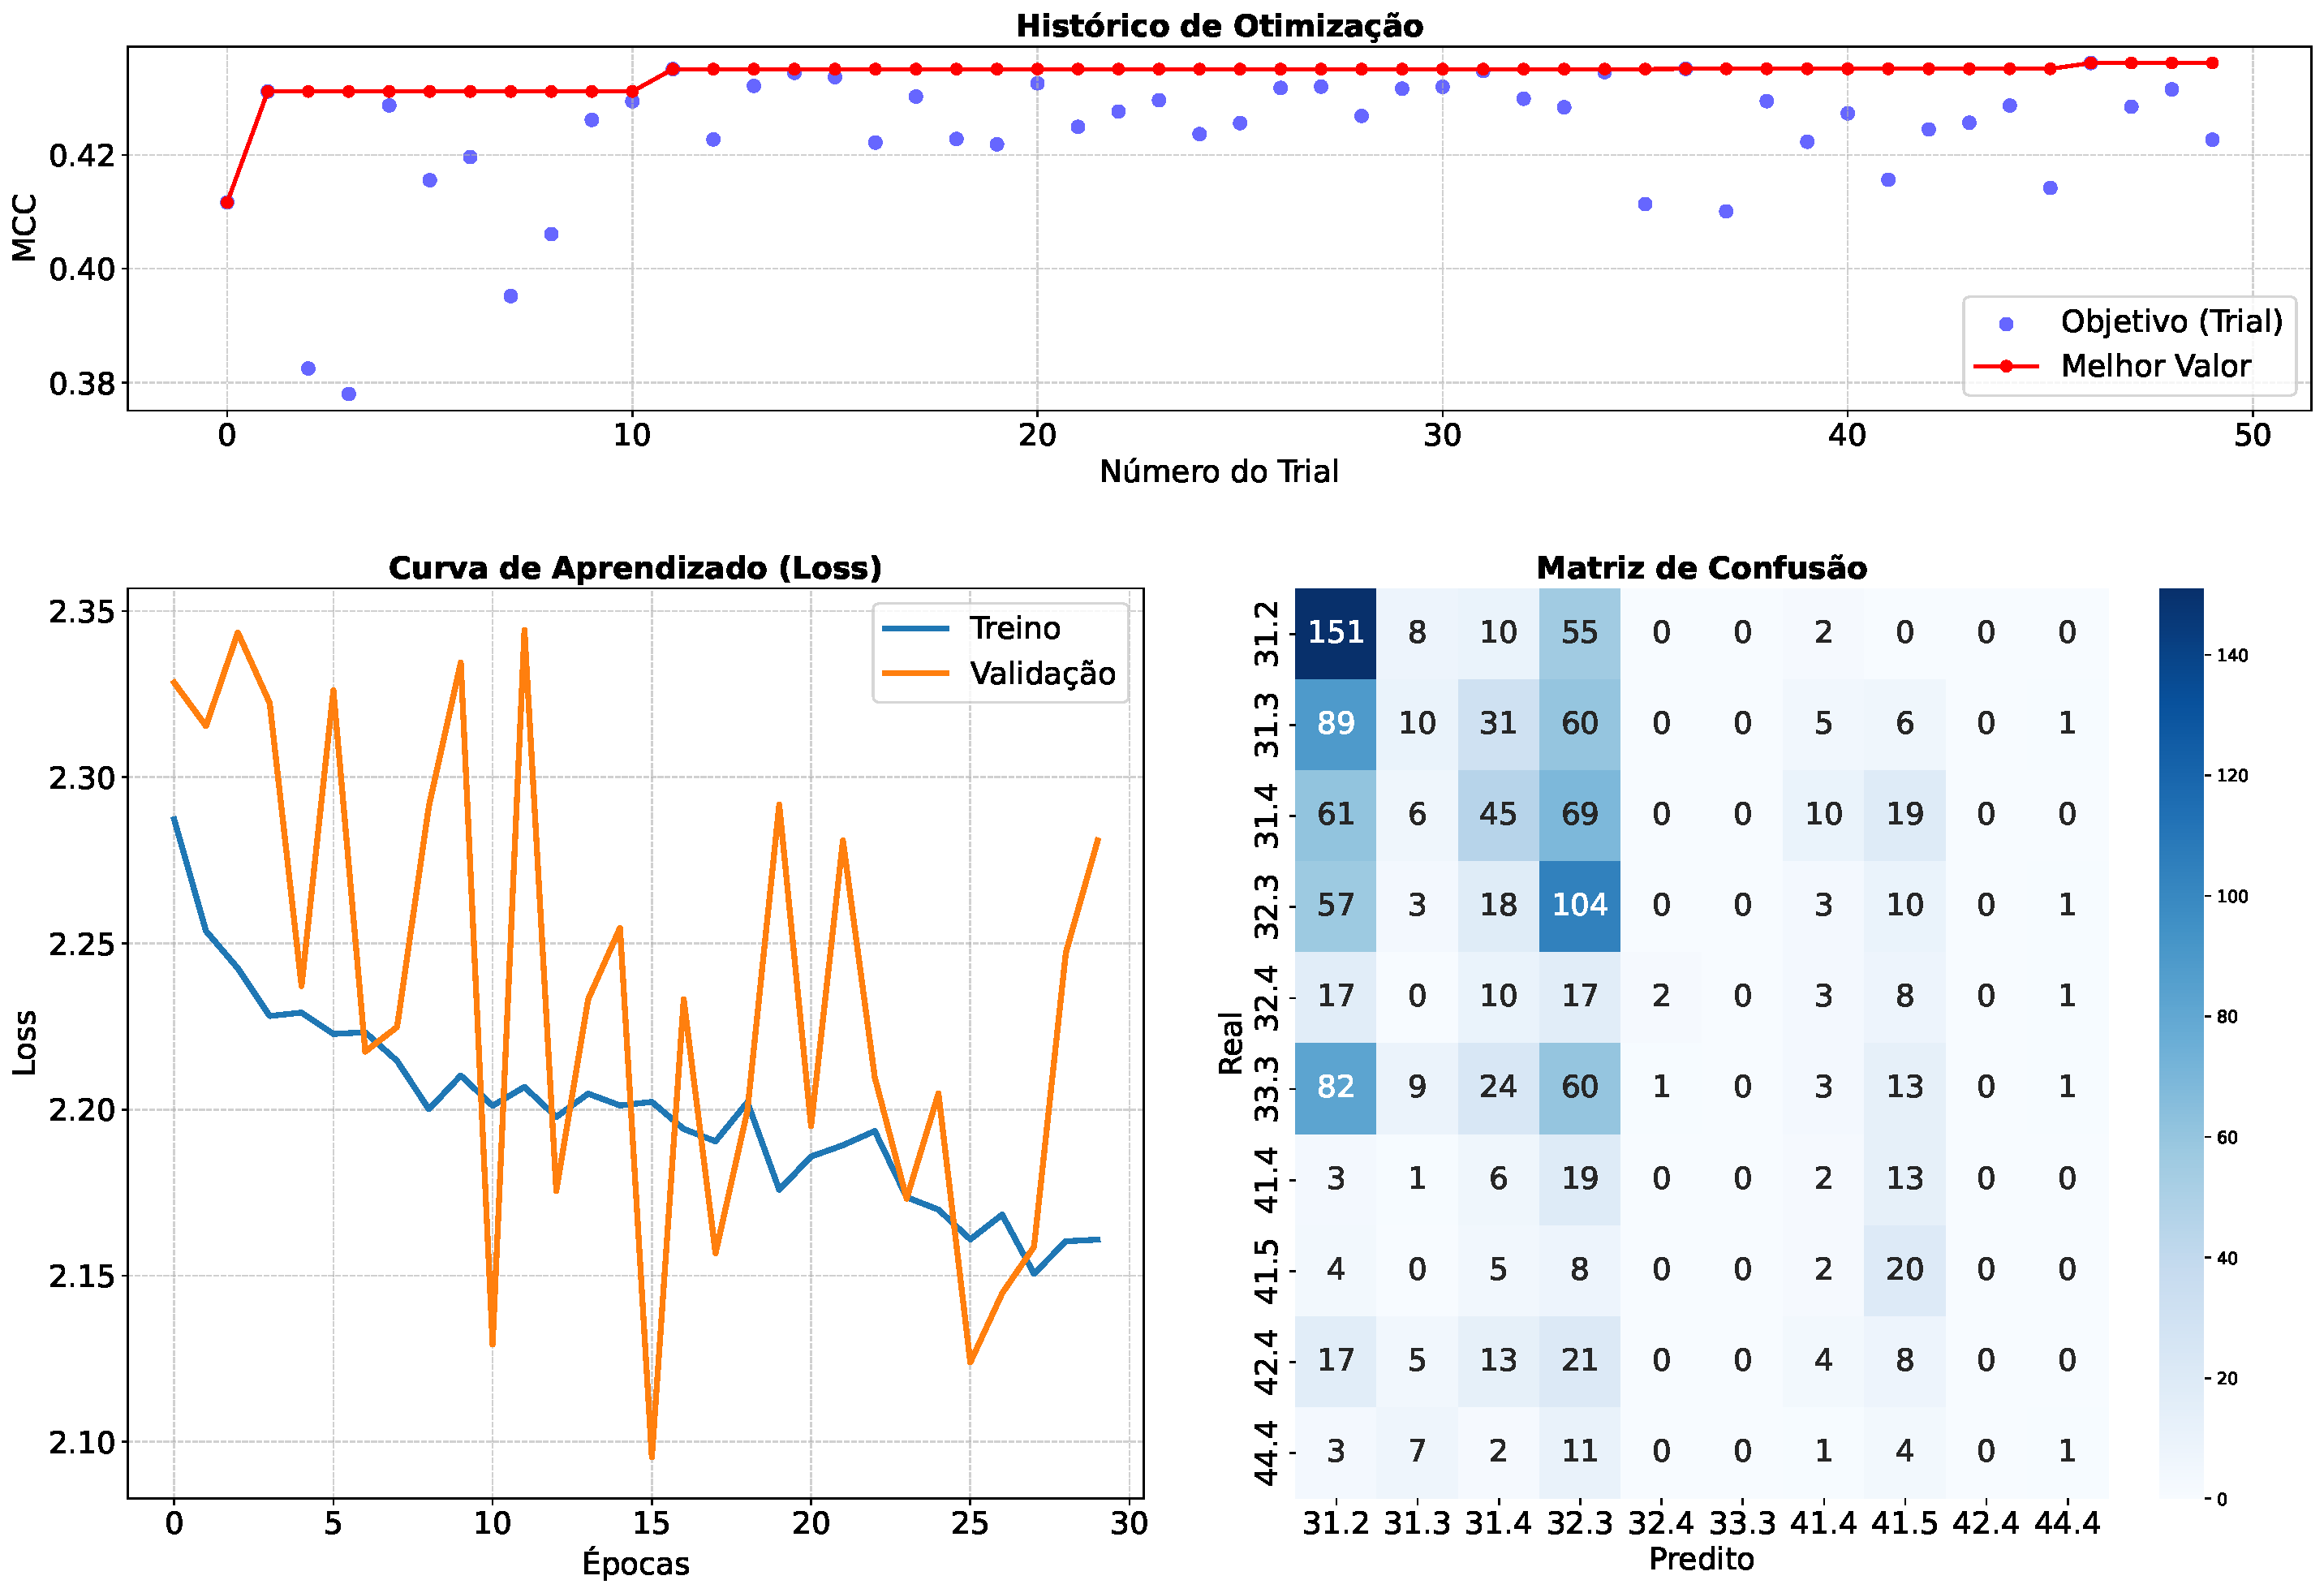
\includegraphics[width=0.85\textwidth]{tex/appendix/experiments/swin_v1_AB_opt/dashboard_consolidado.pdf}
        \caption{Histórico de Otimização, Curvas de Aprendizado e Matriz de Confusão - swin\_v1\_AB\_opt}
    \end{figure}
\end{minipage}
\clearpage
